\chapter{Projektbeschreibung}
% noch mal Bezug nehmen auf das Projektplanungsdokument (nur das, was wirklich relevant
% für dieses Projekt ist)
\section{Ausgangslage und Problemstellung}
Die Ausgangslage dieses Projektes lässt sich durch die dringende Notwendigkeit einer umfassenden Schulung sowie einer anschließenden Zertifizierung zur Einführung des neuen Raumplanungsassistenten RAPLA beschreiben. Dieser Assistent soll den Prozess der Raumplanung erheblich vereinfachen und optimieren. Für die erfolgreiche Einführung ist es jedoch unerlässlich, dass die Nutzerinnen und Nutzer entsprechend geschult und zertifiziert werden. Im Rahmen dieser Gruppenarbeit liegt der organisatorische Schwerpunkt auf der Implementierung der Zertifizierung. Diese wird durch die Entwicklung eines Wissensquizzes und eines abschließenden Zertifizierungsquizzes realisiert. Das zugrunde liegende Projektplanungsdokument hebt hervor, dass die inhaltliche Komplexität des Raumplanungsassistenten RAPLA eine tiefgehende und umfassende Schulung sowie eine präzise Zertifizierung notwendig macht. Daher ist eine strukturierte und detaillierte Herangehensweise erforderlich, um sicherzustellen, dass alle relevanten Aspekte abgedeckt werden und die Nutzerinnen und Nutzer optimal vorbereitet sind.

\section{Anforderungen an das Quiz}
Die Anforderungen an das Quiz sind äußerst vielfältig und umfangreich. Zum einen soll das Quiz die Lernenden auf die bevorstehende Zertifizierung optimal vorbereiten, wobei ein besonderer Fokus auf einer hohen Benutzerfreundlichkeit liegt. Dies bedeutet, dass das Quiz intuitiv und einfach zu bedienen sein muss, um eine positive Lernerfahrung zu gewährleisten. Zum anderen dient das Quiz der Überprüfung des erworbenen Wissens in Bezug auf den gesamten Projektumfang. Hierbei ist es essenziell, dass das Quiz sowohl theoretische Fragen als auch praktische Aufgaben in unterschiedlichen Schwierigkeitsgraden enthält. Diese Fragen und Aufgaben müssen so formuliert sein, dass sie klare und eindeutige Antworten ermöglichen, was eine automatisierte Bewertung erleichtert. Nach der Bewertung soll den Lernenden eine Rückmeldung in Form eines Zertifikates gegeben werden, welches ihren Kenntnisstand offiziell bestätigt.
Für die Umsetzung des Quizzes wird die Lernplattform Moodle genutzt, da diese Plattform zahlreiche Funktionen bietet, die für die Erstellung und Durchführung eines interaktiven und effektiven Quizzes notwendig sind. Moodle ermöglicht es, verschiedene Fragetypen und Aufgabenformate zu integrieren, was zur Vielseitigkeit und Dynamik des Quizzes beiträgt. Darüber hinaus werden zwei reale Rapla-Instanzen zur Darstellung der Aufgaben verwendet. Insgesamt soll das Quiz nicht nur ein hohes Maß an Interaktivität bieten, sondern auch sicherstellen, dass die Lernenden intensiv mit den Inhalten des Raumplanungsassistenten RAPLA vertraut gemacht werden und so bestens auf die Zertifizierung vorbereitet sind.

\section{Methodik und Vorgehensweise}
Die Methodik und Vorgehensweise zur Umsetzung dieses Projektes ist in mehrere Phasen unterteilt, um eine systematische und strukturierte Herangehensweise zu gewährleisten.
In der Projektplanungsphase werden zunächst die Ziele und Aufgaben klar definiert. Ein detaillierter Zeitplan wird erstellt, der die verschiedenen Meilensteine des Projektes festlegt. Hierzu gehören unter anderem die Analyse, das Design, die Implementierung, das Testen und die finale Evaluierung.
Während der Analysephase wird eine umfassende Bedarfsanalyse durchgeführt, um die spezifischen Anforderungen an das Quiz zu ermitteln. Dies umfasst die Identifizierung der zu vermittelnden Inhalte sowie die Festlegung der Kriterien für die Zertifizierung. Die Anforderungsanalyse hilft dabei, die notwendigen Funktionalitäten und Eigenschaften des Quizzes zu bestimmen.
In der Designphase wird ein detailliertes Konzept für das Quiz entwickelt. Dies beinhaltet sowohl die inhaltliche Gestaltung als auch die Benutzeroberfläche. Das Ziel ist es, ein benutzerfreundliches und interaktives Quiz zu entwerfen, das den Lernenden eine effektive Vorbereitung ermöglicht.
Die Implementierungsphase umfasst die tatsächliche Programmierung des Quizzes. Dabei wird das Quiz in die Lernplattform Moodle integriert, die aufgrund ihrer vielseitigen Funktionen und Benutzerfreundlichkeit ausgewählt wurde. In dieser Phase werden die verschiedenen Fragetypen und Aufgabenformate erstellt und in das System eingebunden.
In der anschließenden Testphase wird das Quiz ausführlich getestet. Hierbei liegt der Fokus auf der Benutzerfreundlichkeit und der Funktionalität. Fehler und Probleme werden identifiziert und behoben, um sicherzustellen, dass das Quiz reibungslos funktioniert.
Die Evaluierung und Feedback-Phase beinhaltet das Sammeln von Rückmeldungen der ersten Nutzer. Basierend auf diesem Feedback werden notwendige Anpassungen vorgenommen, um die Qualität und Effektivität des Quizzes weiter zu verbessern.
In der letzten Phase, der Finalisierung und Rollout, wird die Abschlussdokumentation erstellt und das Quiz finalisiert. Zudem erfolgt die Schulung der Trainer, die das Quiz in Zukunft betreuen werden, sowie der offizielle Rollout des Quizzes für alle Nutzer.
Diese strukturierte Vorgehensweise stellt sicher, dass das Projekt methodisch und effizient umgesetzt wird, wodurch die Ziele der Schulung und Zertifizierung des Raumplanungsassistenten RAPLA erfolgreich erreicht werden können.


% Grundsätzlich umfasst das Projektmanagement alle organisatorischen und führungsrelevanten Aufgaben
% sowie Techniken und Mittel zur operativen Durchführung, Überwachung und
% Unterstützung von Projekten.
% \footcite[Vgl.][3]{holzbaurNachhaltigesProjektmanagementVerantwortlichkeit2022}
% Insbesondere die Qualität eines Projekts ist abhängig
% von der Beschaffenheit des Projektmanagements.
% \footcite[Vgl.][52]{stoegerWirksamesProjektmanagementMit2019}
% Eine der Kerndisziplinen des
% Projektmanagements ist die Projektorganisation, welche Projektpläne,
% Dokumentationen für Projektmitarbeiter, eine Zeitplanung sowie
% die Verteilung von Aufgabenpaketen und jegliche weiteren Formen der
% Projektinfrastruktur umfasst.
% \footcite[Vgl.][53]{stoegerWirksamesProjektmanagementMit2019}
% Ein verbreiteter Ansatz der regelmäßigen Überprüfung der Projektorganisation
% stammt von Peter Drucker und besteht darin, in festgelegten Intervallen
% drei Kernfragen zu beantworten:
% \begin{itemize}
%     \item Ist die Projektorganisation so ausgerichtet, dass Nutzen für den Projektkunden gestiftet wird?\footcite[][57]{stoegerWirksamesProjektmanagementMit2019}
%     \item Stellt die Projektorganisation sicher, dass die Projektmitarbeiter ihre Aufgaben so erledigen können, dass der Zweck des Projekts erreicht wird?\footcite[][57]{stoegerWirksamesProjektmanagementMit2019}
%     \item Kann sich die Projektleitung mithilfe der Projektorganisation ihrer Kernaufgabe widmen – der Steuerung des Projekts?\footcite[][57]{stoegerWirksamesProjektmanagementMit2019}
% \end{itemize}
% \section{Projektplanung und Projektrollen}
% Zu Beginn eines jeden Projekts benötigt es eine Verteilung der Rollen und Verantwortlichkeiten innerhalb des Projekts.
% \footcite[Vgl.][89]{stoegerWirksamesProjektmanagementMit2019}
% In einem Projekt gibt es zahlreiche solcher Stakeholder, deren Identifikation und Management von entscheidender Bedeutung sind.
% Um dies effektiv zu handhaben, empfiehlt es sich, ein strukturiertes Schema zur Erfassung und Organisation dieser Stakeholder zu verwenden.
% Die Blaupause des benutzten Schemas für die Festlegung der Projektrollen und deren Verantwortlichkeiten ist in \textit{Anhang 1} zu finden.
% Die konkrete Zuordnung der Rollen und jeweils verantwortlichen Personen erfolgt hierbei bereits im Vorfeld der Projektplanung
% (siehe Tab. \ref{tab:rollen}).
% \begin{table}[H]
%     \centering
%     \begin{tabular}{|p{3.5cm}|p{4cm}|p{7cm}|}
%         \hline
%         \textbf{Rolle} & \textbf{Besetzung} & \textbf{Verantwortlichkeiten} \\
%         \hline
%         Auftraggeber & Michael Herwig & Auftragserteilung, Vorgabe und Kontrolle \\
%         & Prof. Kai Holzweißig & der Ziele, Abnahme des Projektergebnisses \\ 
%         & Lars Probst & \\
%         \hline
%         Projektleitung & Simon Spitzer & \begin{itemize}
%             \item Ziele der Auftraggeber in Teilziele und Arbeitspakete aufteilen
%             \item Aufgaben, Komeptenzen und Verantwortlichkeiten den Projektmitarbeitern zuordnen
%             \item Projektorganisation und -kommunikationswege festlegen (Jira, Discord, WhatsApp etc.)
%             \item Kommunikation mit Beteiligten (Sekreatariat, Studiengangsleiter etc.)
%             \item Umsetzung des Projektes überwachen und steuern
%             \item Berichterstattung an Auftraggeber
%         \end{itemize} \\
%         % Ziele der Auftraggeber in Teilziele und Arbeitspakete aufteilen \\
%         % & & Aufgaben, Komeptenzen und Verantwortlichkeiten der Projektmitarbeiter festlegen \\
%         % & & Projektorganisation und -kommunikationswege festlegen (Jira, Discord, WhatsApp etc.) \\
%         % & & Kommunikation mit Beteiligten (Sekreatariat, Studiengangsleiter etc.) \\
%         % & & Umsetzung des Projektes überwachen und steuern \\
%         % & & Berichterstattung an Auftraggeber \\
%         \hline
%         Projektmitarbeiter
%         & Simon Burbiel & grundsätzlich Ergebnisse gemäß den \\
%         & Lukas Großerhode & Arbeitspaketen umsetzen und \\
%         & Tim Keicher & verantworten \\
%         & David Stark & \\
%         & Simon Spitzer & \\
%         \hline
%         Externe Experten + & Prof. Kai Holzweißig & \\
%         Vertreter der DHBW & Tanja Schenk & \\
%         & Annette Voellmer & \\
%         & Nicole Bronder & \\
%         \hline
%     \end{tabular}
%     \caption{Rollen und Verantwortlichkeiten im Projekt.}\label{tab:rollen}
% \end{table}
% Besonders hierbei hervorzuheben ist die Kombination der Punkte 4 (externe Experten und Vertreter der DHBW),
% sowie 5. (Kunden). Die als „Experten“ fungierenden Mitarbeiter der DHBW teilen im Rahmen der durchzuführenden Interviews ihre Erfahrungen
% mit dem neuen Raumplanungsassisten und können in diesem Zuge auch auf Besonderheiten hinsichtlich der Nutzung und Bedienbarkeit des Programms
% hinweisen.
% Auch die Perspektiven derjenigen Mitarbeiter,
% welche noch keine Erfahrungen mit RAPLA haben sammeln können, sind von Bedeutung,
% da anhand dieser ebenso neue Erkenntnisse zur Gestaltung der Schulungsunterlagen und
% zur Zertifizierung gewonnen werden können. Des Weiteren ist als Besonderheit hervorzuheben,
% dass die Projektleitung auch operativ im Projekt mitarbeitet und
% sich nicht ausschließlich mit der Projektorganisation und dem Projektmanagement beschäftigt. Obwohl dies in der Literatur nicht in der Form
% angedacht ist, kann es für dieses Projekt unter Berücksichtigung von Umfang und fortlaufender iterativer Weiterentwicklung
% als sinnvoll angesehen werden.
% \footcite[Vgl.][89]{stoegerWirksamesProjektmanagementMit2019}

% \section{Interne Organisationsstruktur}
% Die interne Organisationsstruktur beinhaltet im Wesentlichen Wege der Kommunikation, Prüfungen hinsichtlich des Projektfortschritts,
% Verteilungen von Informationen sowie Möglichkeiten des kollaborativen Zusammenarbeitens.
% \footcite[Vgl.][460]{chenOrganizationalStructureDynamics2015}
% Bereits im Jahr 1996 war bekannt, dass hierfür computergetützte Lösungen vorteilhaft sind.
% \footcite[Vgl.][39]{easonDivisionLabourDesign1996}
% In dem RAPLA Schulungsprojekt wird hierfür das Programm „Jira Software“ benutzt.
% „Jira Software“ ist ein Kollaborationswerkzeug, welches den Nutzern unter anderem die Erstellung von Aufgaben-Übersichtstafeln,
% die Anlage von Listen mit über- und untergeordneten Aufgaben, die Zuordnung von Tätigkeiten zu bestimmten Personen
% sowie die Verwaltung einer Zeitleiste mit Fälligkeitsdaten ermöglicht.
% \footcites[Vgl.][1]{filionUsingAtlassianTools2017}[][87]{rehaPROJECTMANAGEMENTTOOLS2021}[][S. 32 ff.]{bradComparativeStudyAgile}
% Demnach ist dieses Werkzeug optimal für kollaborative Zusammenarbeiten geeignet. Weitere 
% Funktionalitäten und die konkreten Zuständigkeiten werden im Kapitel 
% „Arbeitspaketeplanung“ beschrieben. 

% Als zweites Kollaborationswerkzeug kommt Discord zum Einsatz. Es wird primär für den text- und sprachbasierten Informationsaustausch
% innerhalb des Teams genutzt. Zusätzlich werden dadurch
% Videotelefonate sowie das Teilen persönlicher Bildschirminhalte in Echtzeit ermöglicht.
% Ferner können dedizierte Text-Kanäle erstellt werden, die ebenfalls eine Unterstützung zum Teilen von Dokumenten anbieten.
% Des Weiteren gibt es Sprachkanäle, in welchen Regelmeetings virtuell abgehalten werden können. Eine beispielhafte Struktur eines sogenannten Community-Servers ist im Anhang 2 zu sehen.

% Es können viele Probleme entstehen, wenn vorab keine sinnvolle Verteilung der Aufgaben und Verantwortlichkeiten innerhalb des Teams erfolgt.
% \footcite[Vgl.][122]{suhandaRACIMatrixDesign2021}
% Um diesen Problemen entgegenzuwirken, wird im Rahmen dieses Projekts eine sogenannte \ac{RACI}-Matrix verwendet.
% Durch sie wird sichergestellt, dass alle Tätigkeiten und Rollen den entsprechenden Verantwortlichen zugewiesen werden und etwaige Klärungen hinsichtlich der Verantwortlichkeiten
% im späteren Projektverlauf vermieden werden können.
% \footcite[Vgl.][1]{farnettiOPTIMIZINGCOMMUNICATIONFLOWS2022}
% Die Grundprinzipien der \ac{RACI}-Matrix gehen auf die folgenden vier Buchstaben zurück:
% \begin{itemize}
%     \item \textbf{R}esponsible: Eine Person, welche für die Umsetzung einer Aufgabe verantwortlich ist.\footcite[Vgl.][4]{farnettiOPTIMIZINGCOMMUNICATIONFLOWS2022}
%     \item \textbf{A}ccountable: Eine Person, welche für das finale Endergebnis dem Auftraggeber gegenüber verantwortlich ist.\footcite[Vgl.][4]{farnettiOPTIMIZINGCOMMUNICATIONFLOWS2022}
%     \item \textbf{C}onsulted: Eine Person, welche bspw. aufgrund ihres Fachwissens in Entscheidungsprozesse involviert sein muss.\footcite[Vgl.][4]{farnettiOPTIMIZINGCOMMUNICATIONFLOWS2022}
%     \item \textbf{I}nformed: Eine Person, welche lediglich über den Fortschritt einer Aufgabe informiert werden muss.\footcite[Vgl.][4]{farnettiOPTIMIZINGCOMMUNICATIONFLOWS2022}
% \end{itemize}
% \begin{figure}[H]
%     \centering
%     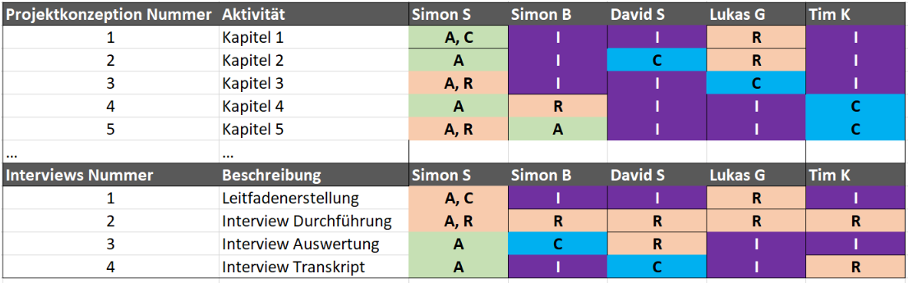
\includegraphics[width=0.9\linewidth]{graphics/raci.png}
%     \caption[Die \ac{RACI}-Matrix des Projekts.]{Die \ac{RACI}-Matrix des Projekts.}\label{abb:raci}
% \end{figure}
% \section{Regelmäßiger Austausch}
% Unabhängig davon, ob es sich um neue Entwicklungen, strategische Überlegungen, operative Angelegenheiten oder allgemeine Probleme handelt,
% ist es unerlässlich, diese Themen zu diskutieren. Dafür können entweder direkt die Verantwortlichen angesprochen werden, wenn diese
% existieren oder aber es wird in Regelmeetings über diese Punkte gesprochen. Jedoch führen ineffektive Regelmeetings zu verspäteten Entscheidungen,
% verschwendeten Ressourcen, verpassten Möglichkeiten und jeder Menge verlorener Zeit. 
% Eine Strategie und Grundsätze für Regelmeetings in einem Projekt zu etablieren und eine gewisse Qualität zu haben,
% scheint daher grundsätzlich vorteilhaft zu sein. Michael C. Mankins hat in seinem Artikel im „Harvard Business Review“-Journal „Stop Wasting Valuable Time” sieben Regeln
% aufgestellt, diese möglichst effektiv zu gestalten:
% \begin{itemize}
%     \item \textbf{Strategie und Operationen getrennt behandeln:} Strategische Themen benötigen mehr Zeit und sollten daher in separaten Meetings behandelt werden.
%     \item \textbf{Fokus auf Entscheidungen, nicht Diskussionen:} Qualität und Geschwindigkeit der Entscheidungsfindung verbessern, indem beispielsweise Dokumente im Voraus verschickt werden. Dies spart jedem Teilnehmer viel Zeit und auch die Gesamtlänge des Meetings wird verkürzt.
%     \item \textbf{Den wirklichen Wert jedes Tagesordnungspunktes messen:} Priorisieren der Tagesordnungspunkte nach ihrer Auswirkung auf den weiteren Verlauf des Projektes. Wichtige Punkte zuerst behandeln.
%     \item \textbf{Themen schnell von der Tagesordnung abhandeln:} Klare Zeitpläne festlegen, wann und wie Teilnehmer jedes Thema entscheiden, damit nicht zu viel Zeit auf einem Thema benötigt wird.
%     \item \textbf{Entscheidungen verbindlich machen:} Explizit vereinbaren, was in der Besprechung entschieden wurde. Entweder direkt während des Meetings festhalten oder eine Kommunikation im Nachgang senden.
% \end{itemize}
% Nachdem ein paar Grundsätze festgelegt werden, geht es an die Feinplanung der 
% Regelmeetings. Im 5. Semester ist ein wöchentliches Meeting jeden Donnerstag um 16:30Uhr vorgesehen.
% Der Zeitumfang beträgt dabei immer maximal eine Stunde. Wenn an diesem Tag Vorlesungen sind, wird werden die Treffen in Präsenz
% im Anschluss an die Vorlesung durchgeführt, in anderen Fällen finden diese per Videokonferenz statt. Zusätzlich zu diesem festgelegten Termin wird in der Vorlesungszeit
% des Kurses „Projektkonzeption“ über operative Tätigkeiten im Detail gesprochen und sich mit dem verantwortlichen Teammitgliedern abgestimmt,
% um die Entstehung von Dupletten oder unbehandelten Punkten am Ende des Projekts zu vermeiden.
